% Write the full path to the location of the graphics relative to book.tex
\graphicspath{{chapters/marcibal/graphics/}} 

\title{Implementation of the Lam-Bremhorst \texorpdfstring{\(k\)-\(\varepsilon\)}{k-e} turbulence model in FEniCS}
\titlerunning{Implementation of the \texorpdfstring{\(k\)-\(\varepsilon\)}{k-e} turbulence model}

\author{Juraj Marcibál, Hans Joachim Schroll}
\authorrunning{J.~Marcibál, H.~J.~Schroll}

\institute{
J.~Marcibál \email{juraj.marcibal@gmail.com},
H.~J.~Schroll \email{achim@imada.dk} 
\at University of Southern Denmark, Department of Mathematics and Computer Science
}

\maketitle

% ---- Article starts here ---- 

% Abstract
\abstract{
In this paper, we give an overview of turbulence modeling and turbulence in general, followed by an implementation of the Lam-Bremhorst \(k\)-\(\varepsilon\) turbulence model in FEniCS \citep{alnaes2015fenics,baratta2023dolfinx}. We demonstrate how the model can be easily implemented in the latest version of FEniCS, even when working with the simplest methods and schemes. We hope this paper serves as a valuable resource for researchers and enthusiasts seeking a straightforward introduction to turbulence modeling and a practical guide for implementing models in FEniCS.
}

% Section 1 - Introduction
\section{Introduction and governing equations}

Turbulence is an ever-present phenomenon encountered in both natural environments and engineering systems, from airflow over an airplane wing to the movement of water in rivers. It occurs when fluid moves chaotically, irregularly and at a high Reynolds number, presenting challenges for study and applications \citep{wilcox_turbulence_2006}. 

\subsection{Literature review}

Turbulence modeling, including the \(k\)-\(\varepsilon\) model and implementation in FEniCS and other open-source software, has been covered in the literature before. The article by \cite{valen_implementing_2013} implements the model by \citep{launder_application_1974}, which is often regarded as the standard \(k\)-\(\varepsilon\) model, in FEniCS, providing an accessible introduction to turbulence modeling and FEniCS itself. However, the provided code is now over a decade old and only covers a simple channel flow case. 

On the other hand, \cite{mortensen_fenics-based_2011} present a more comprehensive turbulence modeling framework, implementing multiple models, including the Launder-Sharma \(k\)-\(\varepsilon\) model. While it extends beyond the turbulent channel flow example, the code is also incompatible with the latest version of Legacy FEniCS and its complexity makes it less approachable for newcomers.

This article aims to address the need for a clear up-to-date turbulence model implementation in the Legacy FEniCS. We demonstrate that implementing a turbulence model in the latest version is feasible, and satisfactory results can be obtained even when working with simple numerical schemes and simpler turbulence model. Additionally, we provide an introduction to turbulence and turbulence modeling, making this work a valuable starting point for researchers entering the field. 

\subsection{Modeling turbulence}

Consider the incompressible Navier-Stokes (N-S) equations
\begin{equation}\label{eq: N-S}
    \begin{split}
        \frac{\partial \mathbf{u}}{\partial t} + \mathbf{u} \cdot \nabla{\mathbf{u}}
        = 
        - \frac{1}{\rho} \nabla p + \nabla \cdot (\nu \nabla \mathbf{u}) + \mathbf{f},
        \\
        \nabla \cdot \mathbf{u}
        = 0,
    \end{split}
\end{equation}
where \(\mathbf{u}\), \(p\) are the instantaneous velocity and pressure, \(\mathbf{f}\) represents the external forces, \(\rho\) is the density and \(\nu\) is the molecular viscosity of the fluid. It is well known that solving Equation \eqref{eq: N-S} numerically becomes difficult as Reynolds Number gets large. To accurately predict turbulent flow, we either need to work with a very fine mesh and small step-size, or resort to modeling. The former is often not feasible without a large computational power.

One approach to modeling turbulence is to consider not the instantaneous \(\mathbf{u}\) and \(p\), but rather the mean values \(\langle \mathbf{u} \rangle\) and \( \langle p \rangle\). By decomposing \(\mathbf{u}\) and \(p\) into their mean and fluctuating parts \(\mathbf{u} = \langle \mathbf{u} \rangle + \mathbf{u}'\) and \(p = \langle p \rangle + p'\), one can derive governing equations for the mean quantities. Such equations are called the Reynolds-Averaged Navier-Stokes (RANS) equations, and they take the form
\begin{equation}\label{eq: RANS}
    \begin{split}
        \frac{\partial \langle \mathbf{u} \rangle}{\partial t} + \langle \mathbf{u} \rangle \cdot \nabla{\langle \mathbf{u} \rangle}
        = 
        -\frac{1}{\rho} \nabla \langle p \rangle + \nabla \cdot (\nu \nabla \langle \mathbf{u} \rangle ) + \langle \mathbf{f} \rangle - \nabla \cdot \langle \mathbf{u}' \otimes \mathbf{u}' \rangle,
        \\
        \nabla \cdot \langle \mathbf{u} \rangle 
        = 0,
    \end{split}
\end{equation}
where \(\mathbf{R} := - \langle \mathbf{u}' \otimes \mathbf{u}' \rangle\) is the Reynolds stress tensor, often interpreted as describing the effect of turbulence on the mean flow \citep{wilcox_turbulence_2006}. It contains \(\mathbf{u}'\) which is not known nor solved for. The RANS equations are therefore not closed and \(\mathbf{R}\) needs to be modeled, usually using the hypothesis proposed by \cite{boussinesq__essai_1877}:
\begin{equation}\label{eq: Boussinesq hypothesis}
    \mathbf{R} 
    \approx 
    - \frac{2}{3}k \mathbf{I} 
    + \nu_t \left(\nabla{\mathbf{u}} 
    + (\nabla{\mathbf{u}})^T\right)
    \implies
    \nabla \cdot \mathbf{R} 
    \approx
    - \frac{2}{3} \nabla k 
    + \nabla \cdot \left( \nu_t \nabla \mathbf{u} \right),
\end{equation}
where \(\nu_t\) is the turbulent viscosity and \(k\) is the turbulent kinetic energy. Modeling turbulence now reduces to modeling \(\nu_t\) and \(k\), usually by solving additional transport equation or equations, one of them typically being a transport equation for \(k\).

\subsection{The Lam-Bremhorst \(k\)-\(\varepsilon\) model and boundary conditions}

The Lam-Bremhorst (L-B) \(k\)-\(\varepsilon\) model \citep{lam_modified_1981} is one of the models proposed to close the RANS equations. It was chosen for its relative simplicity compared to the more popular models such as the model by \cite{launder_application_1974}. Formulated in Equation \eqref{eq: k-eps}, it supplements Equations \eqref{eq: RANS}, \eqref{eq: Boussinesq hypothesis} with two additional transport equations governing \(k\) and \(\varepsilon\) (dissipation of \(k\)). Together, these equations form a closed system that describes the mean behavior of turbulent flow.
\begin{equation}\label{eq: k-eps}
    \begin{split}
        &\frac{\partial \mathbf{u}}{\partial t} 
        + \mathbf{u} \cdot \nabla{\mathbf{u}}
        = 
        - \nabla{\left( \frac{1}{\rho}p + \frac{2}{3}k \right)}
        + \nabla \cdot \left[ (\nu + \nu_t) \nabla \mathbf{u} \right]
        + \mathbf{f},
        \\
        &\nabla \cdot \mathbf{u}
        = 0,
        \\
        &\frac{\partial k}{\partial t} 
        + \mathbf{u} \cdot \nabla{k}
        = \nabla \cdot \left[\left(\nu + \frac{\nu_t}{\sigma_k}\right) \nabla{k} \right]
        + P_k
        - \gamma k,
        \\
        &\frac{\partial \varepsilon}{\partial t} 
        + \mathbf{u} \cdot \nabla{\varepsilon}
        = \nabla \cdot \left[\left(\nu + \frac{\nu_t}{\sigma_\varepsilon}\right) \nabla{\varepsilon}\right]
        + C_1 f_1 P_k \gamma
        - C_2 f_2 \gamma \varepsilon,
        \\
        &\nu_t
        = C_\nu f_\nu \frac{k^2}{\varepsilon},
        \quad 
        P_k 
        = \mathbf{R} : \frac{1}{2} \left(\nabla{\mathbf{u}} + (\nabla{\mathbf{u}})^T\right),
        \quad
        \gamma
        = \frac{\varepsilon}{k},
        \\
        &f_\nu
        = (1 - \exp{\left( -0.0165 \text{Re}_k \right)})^2 \left(1 + \frac{20.5}{\text{Re}_\ell}\right),
        \quad
        f_1
        = 1 + \left( \frac{0.05}{f_\nu}\right)^3,
        \\
        &f_2 
        = 1 - \exp{\left(-\text{Re}_\ell^2\right)},
        \quad
        \text{Re}_k 
        = \frac{\sqrt{k} y}{\nu}, 
        \quad
        \text{Re}_\ell
        = \frac{k^2}{\nu \varepsilon},
        \\
        &C_\nu = 0.09, \quad
        C_1 = 1.44, \quad
        C_2 = 1.92, \quad
        \sigma_k = 1.0, \quad
        \sigma_\varepsilon = 1.3.
    \end{split}
\end{equation}
In Equation \eqref{eq: k-eps}, \(\mathbf{u}\) and \(p\) are the mean velocity and pressure (for better readability we no longer denote averages with \(\langle \cdot \rangle\)), \(k\) and \(\varepsilon\) are the turbulent kinetic energy and its dissipation, \(\rho\), \(\nu\) and \(\mathbf{f}\) are as in Equation \eqref{eq: N-S}. Additionally, \(\nu_t\) is the turbulent viscosity, \(P_k\) and \(\gamma\) are the production and reaction terms of \(k\). 

On top of that \(f_\nu\), \(f_1\) and \(f_2\) are the damping functions, which solve the models' inability to predict flow near the wall \citep{greenshields_notes_2022}. Terms \(\text{Re}_k\) and \(\text{Re}_\ell\) are both referred to as the turbulent Reynolds numbers and \(y\) denotes the distance to the nearest solid wall. Lastly, \(C_\nu\), \(C_1\), \(C_2\) and \(\sigma_1\), \(\sigma_2\) are the experimentally determined model constants.

Since RANS and the N-S are the same equations with different total pressure and total viscosity terms, they also have similar boundary conditions, hence we will only focus on boundary conditions for the equations governing \(k\) and \(\varepsilon\).

For \(k\) and \(\varepsilon\) consider the domain boundary \(\partial \Omega\) divided into disjoint subboundaries corresponding to solid walls, inflow and outflow. Natural boundary conditions for the outflow for both \(k\) and \(\varepsilon\) are the zero Neumann boundary conditions, i.e. \(\nabla k \cdot \mathbf{n} = 0\) and \(\nabla \varepsilon \cdot \mathbf{n} = 0\). For the solid wall \(k\) is set to zero, the boundary conditions for \(\varepsilon\) differs with different turbulence model, for the L-B \(k\)-\(\varepsilon\) model we have \(\nabla \varepsilon \cdot \mathbf{n} = 0\). The inflow boundary conditions are most often estimated from the physical definitions of \(k\) and \(\varepsilon\):
\begin{equation*}\label{eq: definitions of k-e}
    k = \frac{3}{2} (U I)^2, 
    \quad
    \varepsilon = C_\nu \frac{k^{3/2}}{\ell},
\end{equation*}
where \(U\) is the average velocity magnitude, \(I\) is the turbulent intensity and \(\ell\) is the turbulent length scale. Both \(I\) and \(\ell\) are generally not known beforehand and need to be estimated. For estimation of \(I\) and \(\ell\) see \cite{greenshields_notes_2022}. These can then be implemented as Dirichlet boundary conditions in Legacy FEniCS.

\subsection{Non-dimensionalized quantities and the Law of the wall}

In turbulence modeling, many results are formulated using the non-dimensionalized velocity magnitude (\(U^+\)), distance to the wall (\(y^+\)) and turbulent kinetic energy (\(k^+\)) given by:
\begin{equation}\label{eq: non-dimensionalized variables}
    U^+ := \frac{U}{U_\tau},
    \quad
    y^+ := \frac{y U_\tau}{\nu},
    \quad
    k^+ := \frac{k}{U_\tau^2},
\end{equation}
where \(U_\tau := \sqrt{\tau_\text{w}}\) is the so-called friction velocity and \(\tau_\text{w}\) is the so-called wall shear stress, in \(2\)D it is given by \( \tau_\text{w} := \left. \nu [\nabla (\mathbf{u} \cdot \mathbf{t})] \cdot \mathbf{n} \right\rvert_\text{wall} \), where \(\mathbf{n}\) and \(\mathbf{t}\) are the unit outward-facing normal and unit tangent vectors respectively. Note that in \(3\)D the definition of \(\tau_\text{w}\) is more complicated because of non-uniqueness of a tangent vector to the wall. We will however keep the test cases in this paper to \(2\)D only.

% Section 2 - Implementation
\section{Implementation}

In this section, we focus on the implementation of the L-B \(k\)-\(\varepsilon\) model. We only outline the implementation of the transport equations for \(k\) and \(\varepsilon\), since the RANS equations can be solved using the same techniques as N-S. In our case we used Chorin's splitting method together with Taylor-Hood elements to solve the transient version of RANS equations. For the steady state version, Picard iteration was used. 

\subsection{Weak formulation of the \texorpdfstring{\(k\)-\(\varepsilon\)}{k-e} transport equations}

To derive the weak formulation for the \(k\) equation, we first approximate the temporal derivative \(\partial k / \partial t\) by its finite difference approximation. The entire equation is then multiplied by a test function \(\varphi\). Lastly, the divergence theorem is applied to the diffusion term and zero Neumann boundary conditions are considered, resulting in Equation \eqref{eq: Transport equation for k}. The weak formulation then reads: at each time step \(n+1\) find \(k^{n+1} \in V_{k,\triangle} \subseteq V_k = H^1(\Omega)\) such that:
\begin{equation}\label{eq: Transport equation for k}
    \begin{split}
        &\int_{\Omega} \frac{k^{n+1} - k^n}{\Delta t} \varphi \dx 
        + \int_{\Omega} \left( \mathbf{u}^{n+1} \cdot \Grad k^{n+1} \right) \varphi \dx
        \\
        =
        - &\int_{\Omega} \left( \nu + \frac{\nu_t}{\sigma_k}\right) \Grad k^{n+1} \cdot \Grad \varphi \dx 
        + \int_{\Omega} P_k \varphi \dx 
        - \int_{\Omega} \gamma k^{n+1} \varphi \dx,
    \end{split}
\end{equation}
where \(V_{k, \triangle}\) is the finite element subspace of \(V_k\). The same can be performed for the \(\varepsilon\) transport equation. Both \(V_{k, \triangle}\) and \(V_{\varepsilon, \triangle}\) are spaces of piece-wise linear functions.

Terms \(\nu_t\), \(P_k\), \(\gamma\) and \(f_\nu, f_1, f_2\) are all sources of both non-linearity and coupling, as they all depend on both \(k\) and \(\varepsilon\). If we want to solve the equations separately, using linear solvers, it is most natural to treat all the terms above explicitly, i.e. to compute them using values from the previous time-step. 

\subsection{Further treatment of the equations}

As physical quantities, \(k\) and \(\varepsilon\) only attain positive values. However, the equations as of right now might produce negative values for both. The natural solution is to bound them from below by a small constant \citep{lew_note_2001}. To prevent instabilities, it is also advised to limit \(f_\nu\) to its physical bounds \citep{schimdt_two-equation_1988}:
\begin{equation*}\label{eq: Physical bound of fnu}
    f_\nu \longrightarrow \min(\max(0.01116225, f_\nu), 1.0).
\end{equation*}
It has been observed that the effect of \(k\) in the total pressure term is negligible when compared to the effect of pressure \(p\) or the viscous effects \citep{Ansys_Best_Practice}. On top of that, implementing the \(\nabla k\) term in the RANS equations often leads to instabilities. We therefore decided to omit the \(k\) term altogether from \(\mathbf{R}\):
\begin{equation*}\label{eq: Removing k from R}
    \mathbf{R} \longrightarrow \nu_t \left( \Grad \langle u \rangle + \left( \Grad \langle u \rangle \right)^T \right).
\end{equation*}
This results in a formulation which closer resembles ones found in the literature, as seen in articles by \cite{valen_implementing_2013} or \cite{greenshields_notes_2022}.

\subsection{Computational mesh and distance from the wall}

The \(k\)-\(\varepsilon\) model, as formulated in this article, solves the governing equations up to the solid walls. As we will see in the Results section, the turbulent quantities \(k\) and \(\varepsilon\) display large sensitivity and fluctuations in this region, especially in the region where the value of \(y^+\) is less than \(5\) (called the viscous sub-layer). It is essential that this behavior is captured by the model, therefore a mesh fine enough is required. 

Given a desired non-dimensionalized value \(d^+\), we can construct a mesh, such that for each element that lies on the solid wall, the non-dimensionalized distance \(y^+\) between the wall and the furthest point from the wall in the element is less than \(d^+\), by computing the actual distance \(y\) from Equation \eqref{eq: non-dimensionalized variables}. The problem is that the wall shear stress \(\tau_\text{w}\), used in Equation \eqref{eq: non-dimensionalized variables}, is in general not known beforehand and must be estimated. In short, for a pressure-driven turbulent flow, the wall shear stress can be estimated by plugging the solution for Hagen-Poiseuille flow into the definition of \(\tau_\text{w}\). For flow with prescribed inflow velocity profile see \citep{noauthor_cfd_nodate}.

For simple geometries, such as channel flow, the distance from the wall \(y\) can be computed explicitly. When working with more complex geometry, \(y\) must be estimated, for example by solving the so-called Eikonal equation.

% Section 3 - Results
\section{Results}

In this section, we present results obtained for two test cases, namely the fully developed turbulent channel flow and the flow around a backward-facing step. Complete datasets, meshes, codes, and one different case for further exploration are available on the GitHub page of one of the authors \href{https://github.com/joove123/k-epsilon}{https://github.com/joove123/k-epsilon}.

\subsection{Fully developed turbulent channel flow}

A fully developed turbulent channel flow is a high \(\text{Re}\) flow between two infinitely long plates, approximated with a finite mesh of length \(L\) by imposing periodic boundary conditions, separated by a distance \(2H\) as seen in Figure \ref{fig: fully developed turbulent channel flow}. Flow is driven by a constant negative pressure gradient in the direction of the flow, achieved by prescribing \(p\) on the inflow and the outflow as seen in Table \ref{tab: boundary conditions for the channel flow}. The relative simplicity of this essentially one-dimensional problem makes it a perfect test case for verification of the model. Even though the problem attains a steady solution, a transient solver was used to verify its implementation.

\begin{figure}[htbp]
    \centering
    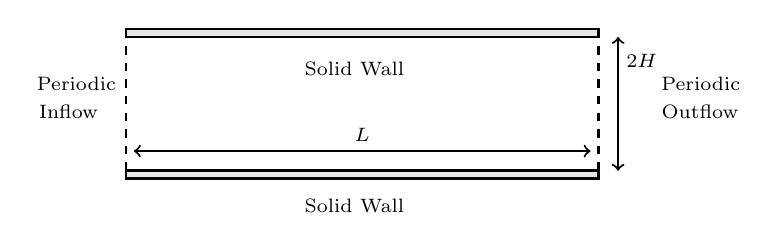
\begin{tikzpicture}
        % Draw a rectangle with specified properties
        \draw[line width=1pt, fill=gray!20] (0.0,1.8) rectangle (6.0,1.9);
        \draw[line width=1pt, fill=gray!20] (0.0,0.0) rectangle (6.0,0.1);
        \draw[dashed, line width=1pt] (0,0.1) -- (0,1.9);
        \draw[dashed, line width=1pt] (6,0.1) -- (6,1.9); 
        
        \node at (2.6+0.3, 1.4) {\scriptsize Solid Wall};
        \node at (2.6+0.3, -0.35) {\scriptsize Solid Wall};
    
        \node at (-0.63, 1.2) {\scriptsize Periodic};
        \node at (-0.73, 0.85) {\scriptsize Inflow};
    
        \node at (7.15+0.15, 1.2) {\scriptsize Periodic};
        \node at (7.15+0.14, 0.85) {\scriptsize Outflow};
    
        % draw arrows
        \draw[<->, line width=0.75pt] (0.1, 0.35) -- (5.9, 0.35);
        \node at (3.0, 0.55) {\scriptsize $L$};
    
        \draw[<->, line width=0.75pt] (6.25, 0.1) -- (6.25, 1.8);
        \node at (6.55, 1.5) {\scriptsize $2H$};
        
    \end{tikzpicture}
    \captionsetup{width=0.85\textwidth}
    \caption{Computational domain for the turbulent channel flow.}
    \label{fig: fully developed turbulent channel flow}
\end{figure}

The simulation is operated at Reynolds number \(\text{Re}_H = 22000\) based on the half-channel height \(H\). However, in turbulence modeling and especially for the turbulent channel flow, the Friction Reynolds number (\(\text{Re}_\tau \)) given by \(\text{Re}_\tau := (U_\tau H) / \nu \) is often used as a measure of the flow. The simulation is operated at \(\text{Re}_\tau = 550\). 

\begin{table}
    \centering
    \begin{tabular}{m{2.1cm} m{1.75cm} m{1.75cm} m{1.75cm} m{1.75cm}}
        \hline
        & $\mathbf{u}$ & $p$ & $k$ & $\varepsilon$ \\
        \hline
        \textbf{Inflow} & periodic & $p=p_{\text{in}}$ & periodic & periodic \\
        \textbf{Outflow} & periodic & $p=p_\text{out}$ & periodic & periodic \\
        \textbf{Solid walls} & $0$ & $\nabla p \cdot \mathbf{n} = 0$ & $0$ & $\nabla \varepsilon \cdot \mathbf{n} = 0$ \\
        \hline
    \end{tabular}
    \captionsetup{width=0.85\textwidth}
    \caption{Boundary conditions for the turbulent channel flow.}
    \label{tab: boundary conditions for the channel flow}
\end{table}

To verify the accuracy of the model, numerical results are compared to a direct numerical simulation performed by \cite{lee_direct_2015}. The same simulation is conducted for a series of meshes with varying values of \(d^+\), ranging from \(16\) to \(0.5\) (smaller value indicates finer mesh), with results provided in Figure \ref{fig: channel flow profiles} (for better clarity, results corresponding to some values of \(d^+\) are not shown). 

\begin{figure}[htbp]
    \centering
    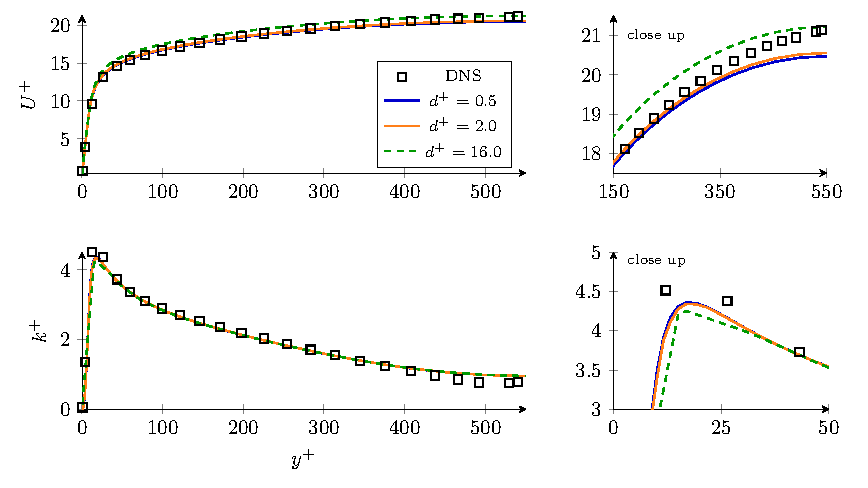
\includegraphics[width=0.825\textwidth]{channel flow-profiles.pdf}
    \captionsetup{width=0.85\textwidth}
    \caption{Comparison of velocity (top) and turbulent kinetic energy (bottom) profiles obtained on meshes with different resolutions with direct numerical simulation (left), together with close-up plots (right).}
    \label{fig: channel flow profiles}
\end{figure}

We feel, considering the solution profiles from Figure \ref{fig: channel flow profiles}, and the fact that the fields are most sensitive in the viscous sub-layer that a value of \(d^+ = 2\) strikes a good balance between computational efficiency and numerical accuracy. For this mesh in particular, number of elements in the mesh is \(864\). Velocity and pressure spaces have \(3480\) and \(511\) degrees of freedom respectively. On the other hand, both \(k\) and \(\varepsilon\) function spaces have \(438\) degrees of freedom. Since results for mesh with value \(d^+ = 2\) and \(d^+ = 0.5\) do not differ dramatically, the former value will also be used when constructing a mesh for the next flow case.  

\subsection{Flow over a backward-facing step}

Flow over a backward-facing step occurs when a fluid flows over a sudden expansion, creating a separated flow region and a complex re-circulation zone downstream of the step. Domain and boundary conditions are constructed such that they match the data from the experiment performed by \cite{driver_features_1985}. Both can be seen in Figure \ref{fig: backward facing step} and Table \ref{tab: boundary conditions for the backward facing step} respectively. This is a significantly more complex scenario than the channel flow, making it a perfect validation case for the model. Because of the mesh size, a steady-state solver was used to obtain the result.    

\begin{figure}[htbp]
    \centering
    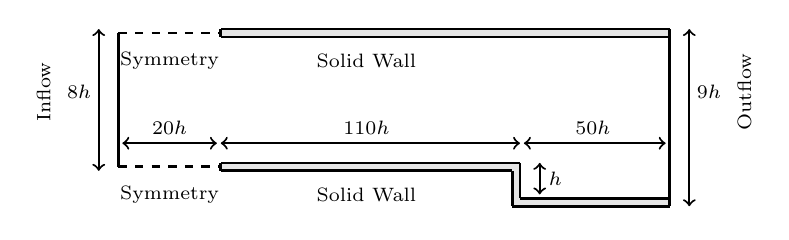
\begin{tikzpicture}
    
        \fill[gray!20] (2.3,1.7) rectangle (8.0,1.8);
        \draw[solid,  line width=1pt]     (2.3,1.7) -- (8.0,1.7);
        \draw[solid,  line width=1pt]     (8.0,1.7) -- (8.0,1.8);
        \draw[solid,  line width=1pt]     (8.0,1.8) -- (2.3,1.8);
        \draw[solid,  line width=1pt]     (2.3,1.8) -- (2.3,1.7);
        
        \fill[gray!20] (2.3,0.0) rectangle (6,0.1);
        \fill[gray!20] (6,-0.45) rectangle (8,-0.35);
        \fill[gray!20] (6,-0.45) rectangle (6.1,0.1);

        \draw[solid,  line width=1.0pt]     (2.3,0.0) -- (6.0,0.0);
        \draw[solid,  line width=1.0pt]     (6.0,0.0) -- (6.0, -0.45);
        \draw[solid,  line width=1.0pt]     (6.0, -0.45) -- (8.0, -0.45);
        \draw[solid,  line width=1.0pt]     (8.0, -0.45) -- (8.0, -0.35);
        \draw[solid,  line width=1.0pt]     (8.0, -0.35) -- (6.1, -0.35);
        \draw[solid,  line width=1.0pt]     (6.1, -0.35) -- (6.1, 0.1);
        \draw[solid,  line width=1.0pt]     (6.1, 0.1) -- (2.3, 0.1);
        \draw[solid,  line width=1.0pt]     (2.3, 0.1) -- (2.3, 0.0);
    
        \draw[dashed, line width=1pt]     (1.,1.75) -- (2.3,1.75);
        \draw[dashed, line width=1pt]     (1.,0.05) -- (2.3,0.05);
        \draw[solid,  line width=1pt]     (1.,0.05) -- (1.,1.75);
        \draw[solid,  line width=1pt]     (8,-0.35) -- (8,1.7);
    
        % Add text labels
        \node at (2.15+2.0, 1.4) {\scriptsize Solid Wall};
        \node at (2.15+2.0, -0.3) {\scriptsize Solid Wall};
    
        \node at (1.65, 1.4) {\scriptsize Symmetry};
        \node at (1.65, -0.3) {\scriptsize Symmetry};
    
        \node[rotate=90] at (0.05, 1.) {\scriptsize Inflow}; 
        \node[rotate=90] at (8.95, 1.) {\scriptsize Outflow};
    
        % draw arrows
        \draw[<->, line width=0.75pt] (6.35, 0.1) -- (6.35, -0.3);
        \node at (6.55, -0.1) {\scriptsize $h$};
    
        \draw[<->, line width=0.75pt] (1.05, 0.35) -- (2.25, 0.35);
        \node at (1.65, 0.55) {\scriptsize $20h$};
        
        \draw[<->, line width=0.75pt] (2.3, 0.35) -- (6.1, 0.35);
        \node at (4.15, 0.55) {\scriptsize $110h$};
        
        \draw[<->, line width=0.75pt] (6.15, 0.35) -- (7.95, 0.35);
        \node at (7.025, 0.55) {\scriptsize $50h$};
    
        \draw[<->, line width=0.75pt] (8.25, -0.45) -- (8.25, 1.8);
        \node at (8.5, 1.) {\scriptsize $9h$};
    
        \draw[<->, line width=0.75pt] (0.75, 0.0) -- (0.75, 1.8);
        \node at (0.5, 1.) {\scriptsize $8h$};
        
    \end{tikzpicture}
    \captionsetup{width=0.85\textwidth}
    \caption{Computational domain for the flow over backward-facing step.} 
    \label{fig: backward facing step}
\end{figure}

The Reynolds number based on the step height \(h\) is approximately \(\text{Re}_h = 36000\), where the reference velocity used to compute \(\text{Re}_h\) is measured just before encountering the step, specifically at \(x = -4h\) (with the step located at \(x=0\)). Computational mesh consists of \(129 844\) elements. There are \(523 038\) and \(65 838\) degrees of freedom for velocity and pressure spaces respectively, and \(65 838\) for both \(k\) and \(\varepsilon\) spaces. 

\begin{table}
    \centering
    \begin{tabular}{m{2.1cm} m{1.75cm} m{1.75cm} m{1.75cm} m{1.75cm}}
        \hline
        & $\mathbf{u}$ & $p$ & $k$ & $\varepsilon$ \\
        \hline
        \textbf{Inflow} & $\mathbf{u}_{\text{in}}$ & $\nabla p \cdot \mathbf{n} = 0$
        & $k_{\text{in}}$ & $\varepsilon_{\text{in}}$
        \\
        \textbf{Outflow} & $\nabla \mathbf{u} \cdot \mathbf{n} = 0$ & $p=0$ 
        & $\nabla k \cdot \mathbf{n} = 0$ & $\nabla \varepsilon\cdot \mathbf{n} = 0$
        \\
        \textbf{Solid walls} & $0$ & $\nabla p \cdot \mathbf{n} = 0$ 
        & $0$ & $\nabla \varepsilon \cdot \mathbf{n} = 0$
        \\
        \textbf{Symmetry} & $\mathbf{u} \cdot \mathbf{n} = 0$ & $\nabla p \cdot \mathbf{n} = 0$ 
         & $\nabla k \cdot \mathbf{n} = 0$ & $\nabla \varepsilon \cdot \mathbf{n} = 0$
        \\
        \hline
    \end{tabular}
    \captionsetup{width=0.85\textwidth}
    \caption{Boundary conditions for the flow over backward-facing step.}
    \label{tab: boundary conditions for the backward facing step}
\end{table}

The model's accuracy is verified using experimental data from \cite{driver_features_1985}. A key measure of success is accurately predicting the reattachment point downstream of the step. This is determined by measuring the point \(\hat{x}\) where the skin friction coefficient (\(C_f\)) is equal zero. In the experiment, this was done using a laser oil-flow interferometer. Another measure for analyzing the results is the pressure coefficient (\(C_p\)). The results in Figure \ref{fig: backstep coefficients} show a poor match between the simulation and experiment, with the reattachment point observed at \(\hat{x} = 6.26 h\) compared to the simulation's \(\hat{x} = 5.0 h\). However, this discrepancy is expected from the \(k\)-\(\varepsilon\) model, which is known to struggle with separation and adverse pressure gradients. When compared to results in article by \cite{steffen_jr._critical_1993} with multiple versions of \(k\)-\(\varepsilon\) model, with reattachment points ranging from \(\hat{x} = 4.9\) to \(\hat{x} = 5.5\), we see a better match.

\begin{figure}[htbp]
    \centering
    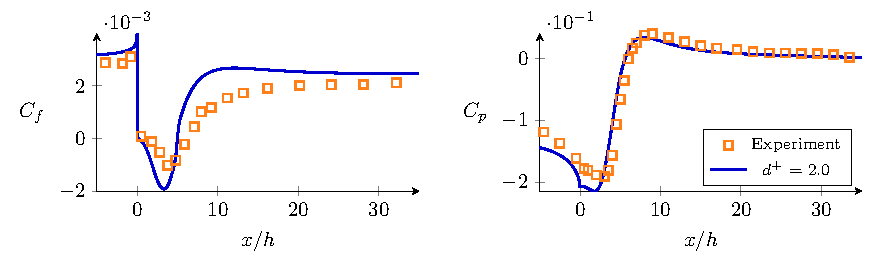
\includegraphics[width=0.825\textwidth]{backstep-coefficients.pdf}
    \captionsetup{width=0.85\textwidth}
    \caption{Comparison of the skin-friction coefficient (left) and the pressure coefficient (right) between experiment and simulation.}
    \label{fig: backstep coefficients}
\end{figure}

Figure \ref{fig: backstep profiles} presents normalized velocity magnitude \(U/U_\infty\) and \(k\) profiles at four points after the step. While the velocity profiles show good agreement, \(k\) diverges after \(x = 4h\), which is likely the cause of the reattachment point appearing prematurely. 

\begin{figure}[htbp]
    \centering
    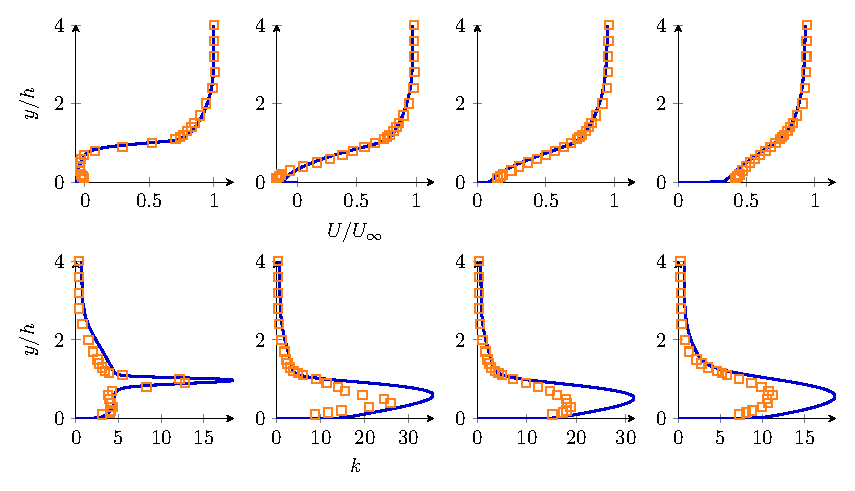
\includegraphics[width=0.825\textwidth]{backstep-profiles.pdf}
    \captionsetup{width=0.85\textwidth}
    \caption{Comparison of velocity (top) and turbulent kinetic energy (bottom) profiles at \(x = 1h\) (left), \(x = 4h\) (second left), \(x = 6h\) (second right) and \(x = 10h\) (right) between experiment and simulation.}
    \label{fig: backstep profiles}
\end{figure}

% Section 4 - Conclusion
\section{Conclusion}

The Lam-Bremhorst \(k\)-\(\varepsilon\) turbulence model was implemented successfully in FEniCS computing platform, both in the transient and steady-state formulation. We verified the implementation of the transient solver by simulating a fully developed channel flow, where a very good agreement was found between the computed solutions and the DNS. While the results of the backward-facing step simulation did not match the experiment, we still consider the implementation of the steady-state solver a success, as the results matched the expected behavior of the \(k\)-\(\varepsilon\) model. It is clear from those results that implementing the working \(k\)-\(\varepsilon\) model in FEniCS can be done with relative ease, and we do not see any reason why that would not be true for different turbulence models such as the \(k\)-\(\omega\) or the Spalart-Allmaras. These results can be replicated via scripts archived at \href{https://github.com/joove123/k-epsilon}{https://github.com/joove123/k-epsilon}.

\begin{acknowledgement}
    I would like to thank my master's thesis supervisor, Prof. Achim Schroll, for his professional guidance and support during the writing of my master's thesis and this article. I also thank NumFOCUS for the travel award that enabled me to attend the FEniCS 2024 conference. 
\end{acknowledgement}

% ---- Article ends here ---- 

\bibliographystyle{spbasic}

% Write the full path of your bibfile relative to book.tex
\bibliography{chapters/marcibal/bibliography.bib}
